
\let\negmedspace\undefined
\let\negthickspace\undefined
\documentclass[journal]{IEEEtran}
\usepackage[a5paper, margin=10mm, onecolumn]{geometry}
%\usepackage{lmodern} % Ensure lmodern is loaded for pdflatex
\usepackage{tfrupee} % Include tfrupee package
\setlength{\headheight}{1cm} % Set the height of the header box
\setlength{\headsep}{0mm}     % Set the distance between the header box and the top of the text
\usepackage{gvv-book}
\usepackage{gvv}
\usepackage{cite}
\usepackage{amsmath,amssymb,amsfonts,amsthm}
\usepackage{algorithmic}
\usepackage{graphicx}
\usepackage{textcomp}
\usepackage{xcolor}
\usepackage{txfonts}
\usepackage{listings}
\usepackage{enumitem}
\usepackage{mathtools}
\usepackage{gensymb}
\usepackage{comment}
\usepackage[breaklinks=true]{hyperref}
\usepackage{tkz-euclide} 
\usepackage{listings}
% \usepackage{gvv}                                        
\def\inputGnumericTable{}                                 
\usepackage[latin1]{inputenc}                                
\usepackage{color}                                            
\usepackage{array}                                            
\usepackage{longtable}                                       
\usepackage{calc}                                             
\usepackage{multirow}                                         
\usepackage{hhline}                                           
\usepackage{ifthen}                                           
\usepackage{lscape}
\renewcommand{\thefigure}{\theenumi}
\renewcommand{\thetable}{\theenumi}
\setlength{\intextsep}{10pt} % Space between text and floats
\numberwithin{equation}{enumi}
\numberwithin{figure}{enumi}
\renewcommand{\thetable}{\theenumi}
\begin{document}
\bibliographystyle{IEEEtran}
\title{10.3.2.2.2}
\author{EE24BTECH11041 - Mohit}
% \maketitle
% \newpage
% \bigskip
{\let\newpage\relax\maketitle}
\begin{enumerate}
\item On comparing the ratios $\frac{a_1}{a_2},\frac{b_1}{b_2}$ and $\frac{c_1}{c_2}$, find out whether the lines representing the following pair of linear equation intersect at a point , are parallel or coincident:\\
\begin{align}
9x + 3y + 12 = 0 \\
18x + 6y + 24 = 0
\end{align}
\textbf{Solution}:-\\
Given,
\begin{align}
a_1=9,b_1=3,c_1=12,a_2=18=b_2=6,c_2=24 \\
\frac{a_1}{a_2}=\frac{b_1}{b_2}=\frac{c_1}{c_2}=\frac{1}{2}
\end{align}
\item Hence,no point of intersect because both lines are same.\\
\textbf{CODING LOGIC}\\



The set of linear equations $9x + 3y + 12 = 0$ and $18x + 6y + 24 = 0$ can be represented by the following equation
\begin{align}
    \myvec{9&3\\18&6}\myvec{x\\y}=\myvec{-12\\-24}
\end{align}
Any non-sigular matrix can be represented as a product of a lower triangular matrix $L$ and an
upper triangular matrix $U$

\begin{align}
    A\vec{x} = LU\vec{x} = \vec{b}
\end{align}
The upper triangular matrix U is found by row reducing A,
\begin{align}
   \myvec{9&3\\18&6} \xrightarrow{R_2 -> R_2 - 2R_1 }\myvec{9&3\\0&0}  
\end{align}
Let 
\begin{align}
    L = \myvec{1 & 0\\ l_{21} & 1}
\end{align}
\begin{align}
l_{21} = A[1][0]=\frac{18}{9}=2
\end{align}


Now,
\begin{align}
    A = \myvec{9&3\\18&6}= \myvec{1 & 0\\ 2 & 1}\myvec{-12\\-24}
\end{align}
Now we can get the solution to our problem by the two step process,
\begin{align}
    L\vec{y} = \vec{b}\\
    U\vec{x} = \vec{y}
\end{align}
Using forward substitution to solve the first equation,
\begin{align}
     \myvec{1 & 0\\ 2 & 1}\myvec{y_1 \\ y_2} &= \myvec{-12\\-24}\\
    \implies \myvec{y_1 \\ y_2} &= \myvec{-12 \\ 0}\\
\end{align}
Now using back-substitution for the second equation,
\begin{align}
    \myvec{9&3\\0&0} \myvec{x_1 \\ x_2} &=  \myvec{-12\\0}
\end{align}
But $U$ is singular, so there is no unique solution.

$\therefore$ The lines $9x + 3y + 12 = 0 $ and $18x + 6y + 24 = 0 $  doesn't intersect.

\end{enumerate}
\begin{figure}[h!]
   \centering
   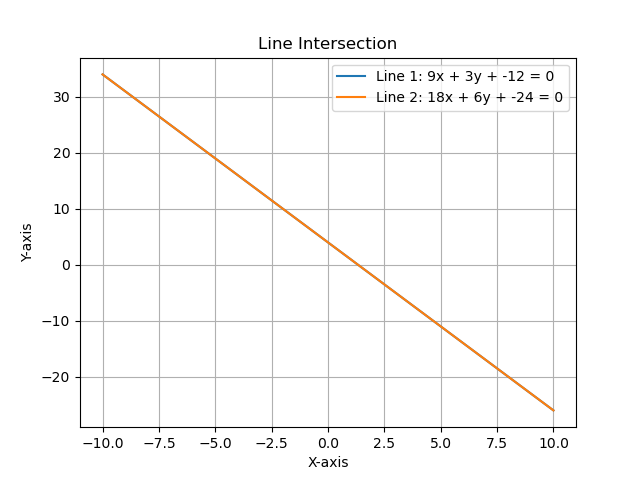
\includegraphics[width=0.7\linewidth]{figs/Figure_1.png}
\end{figure}

\end{document}
